\documentclass[varwidth=40cm]{standalone}
\usepackage{tikz}
\usepackage{style}

\def\tmax{10}

\begin{document}
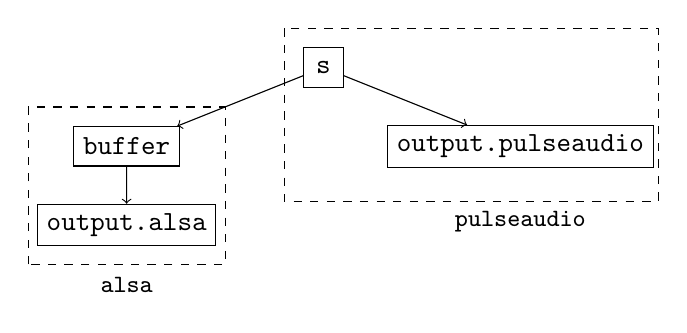
\begin{tikzpicture}[xscale=2.5,minimum size=5mm]
  \node[draw,shape=rectangle] (s) at (0,1) {\texttt{s}};
  \node[draw,shape=rectangle] (buffer) at (-1,0) {\texttt{buffer}};
  \node[draw,shape=rectangle] (alsa) at (-1,-1) {\texttt{output.alsa}};
  \node[draw,shape=rectangle] (pulseaudio) at (1,0) {\texttt{output.pulseaudio}};
  \draw[->] (s) edge (buffer);
  \draw[->] (buffer) edge (alsa);
  \draw[->] (s) edge (pulseaudio);
  \draw[dashed] (-1.5,-1.5) rectangle (-.5,0.5);
  \draw[dashed] (-.2,1.5) rectangle (1.7,-.7);
  \draw (-1,-1.5) node[below] {\small$\texttt{alsa}$};
  \draw (1,-.7) node[below] {\small$\texttt{pulseaudio}$};
\end{tikzpicture}
\end{document}
